\chapter{Versuch 1}

\section{Benötigte Geräte}

Für dieses Experiment benötigen wir die Folgenden Geräte:

\begin{tabular}[h]{c|c|c}
    Gerät & Anzahl & Produktbeeichnung\\
    \hline
    Oszilloskop & 1  & Keysight DSOX1102A\\
    \hline
    Frequenzgenerator & 1 & TELEDYNE T3AFG80\\
	\hline 
	Widerstand 1k & 9 &  \\
	\hline 
	Widerstand 10k & 1 &  \\
	\hline
	Diode & 8 & \\
	\hline
	ADC & 1 & ADC0804LCN \\
	\hline
	Kondesator 0,1 $\mu$ F & 2 & \\
	\hline
	Kondesator 10 $\mu$ F & 1 & \\
	\hline
	Kondesator 150 pF & 1 & 
        \label{tab:Materialliste Versuch 1}
\end{tabular}

\section{Versuchsaufbau}

\begin{center}
	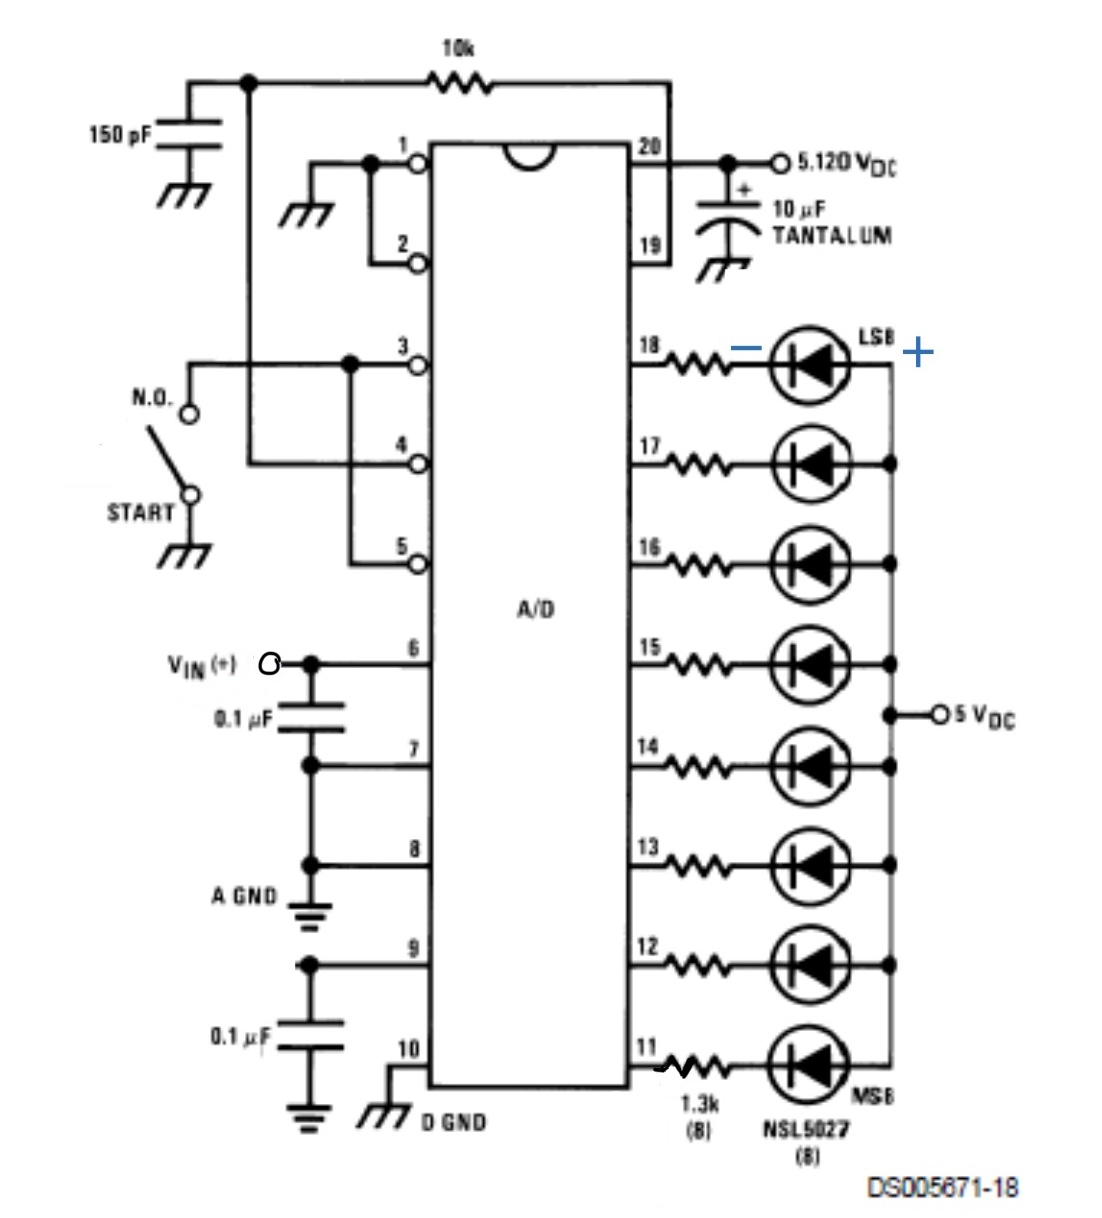
\includegraphics[width=8cm,height=10cm]{images/Schaltungsskizze-versuch-eins.jpg} 
	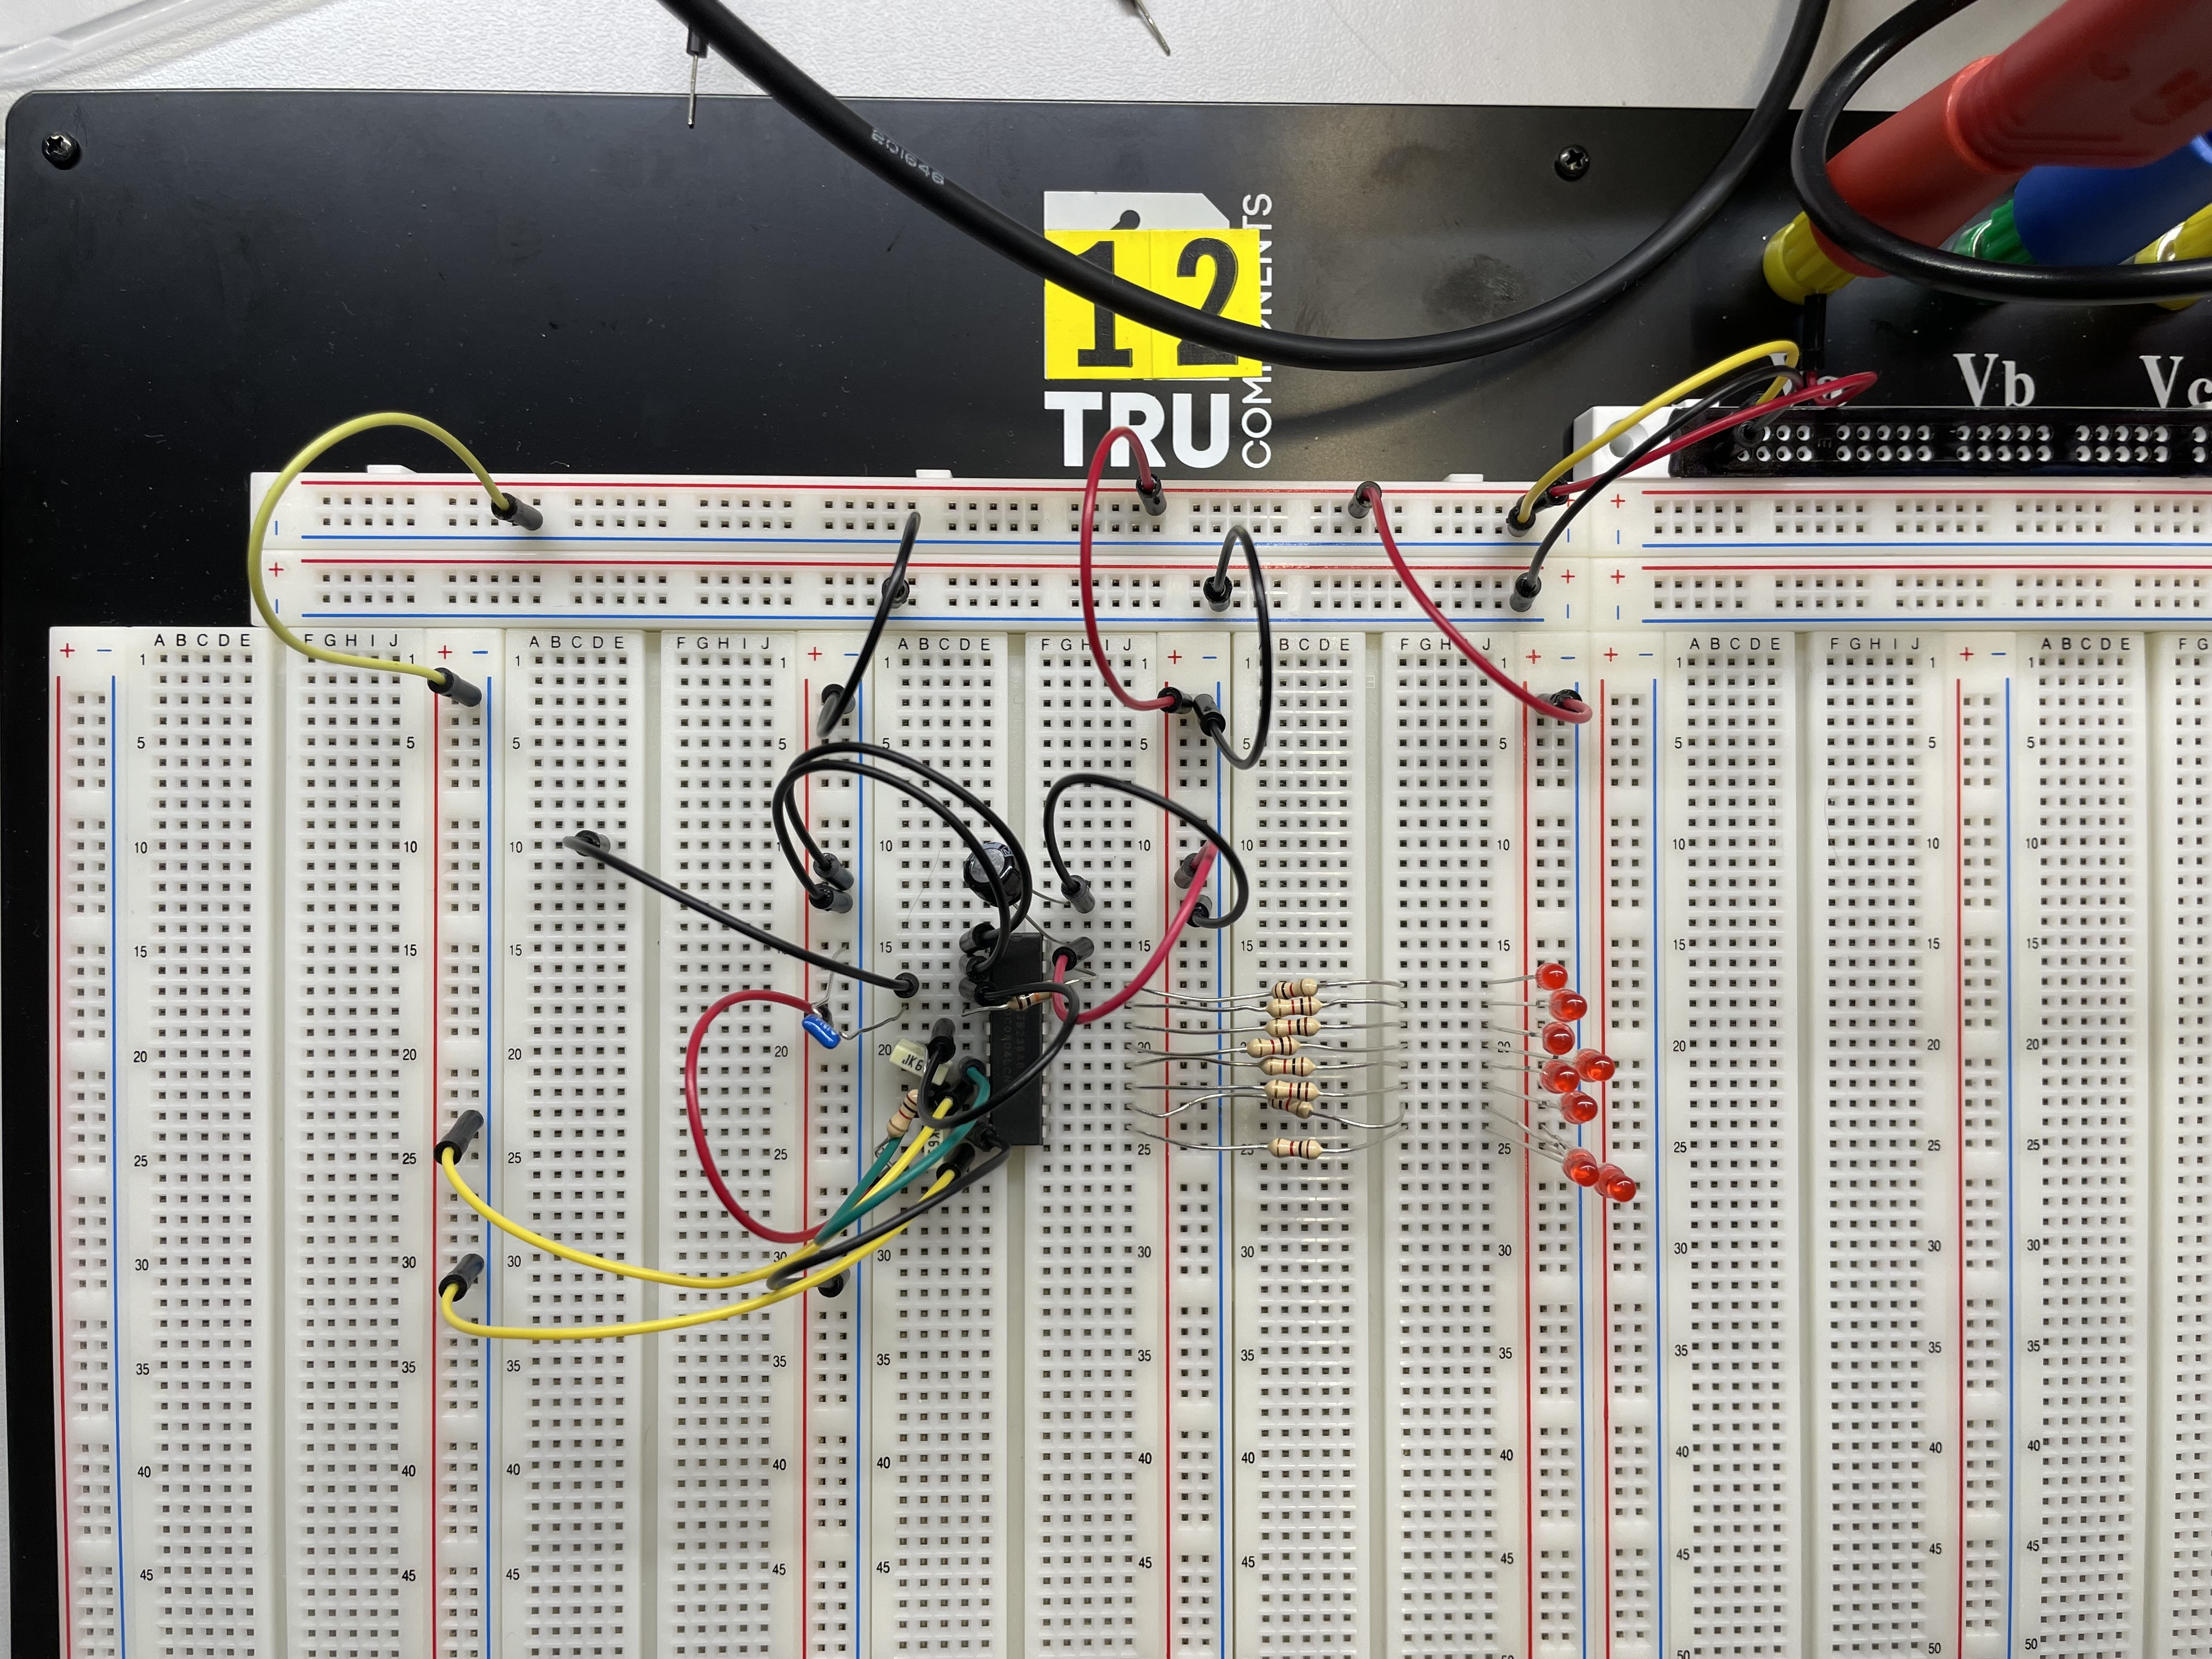
\includegraphics[width=15cm,height=10cm]{images/Schaltungsaufbau-versuch-eins.jpeg}

\end{center}

\section{Integrale Nichtlinearität}
\section{Differentiale Nichtlinearität}
\section{Konversionszeit}
